\section{Voisinages de Margolus}

\par Le voisinage de Margolus est une méthode de voisinage différente du voisinage de Moore, ce qui permet de faire des automates cellulaires différent des algorithmes cellulaires neuraux. Tout comme ce dernier, il existe énormément de règles pour les voisinages de Margolus pouvant être intéressante, par exemple celles de \href{https://dmishin.github.io/js-revca/}{ce site}, dont on a implémenté les règles données.

\subsection{Fonctionnement}

\par Le voisinage de Margolus sont utilisés sur des grilles de taille finie de cases, ou cellules, qui possèdent une valeur qui est soit 0, soit 1, et consistent à regrouper les cellules en groupe de 2x2 cellules, auquel on associe une valeur selon si les cellules du groupe valent 0 ou 1, et cette valeur accompagné par la règle de l'automate cellulaire, remplace le groupe de 2x2 cellules par un autre.

\par Les groupes de 2x2 cellules sont déterminé par leur position, mais aussi par le nombre de générations déjà effectués : à la première génération, on crée les groupe en partant de chaque duos de coordonnées paires : un groupe qui commence en (0,0) (qui englobe donc les cases (0,0), (0,1), (1,0) et (1,1) ), en (0,2), en (2,0) etc... tandis qu'à la seconde génération, On crée les groupes en partant de chaque duos de coordonnées impaires ; on alterne ensuite entre chaque génération. A noter que dans le cas de notre implémentation, des cellules situé sur bord de la grille peuvent créer un groupe avec des cellules situé sur le bord opposé de la grille ; Ainsi si la grille a une taille paire, toutes les cellules feront partie d'un groupe à chaque génération.

\par La façon dont les valeurs sont calculées est similaire à du binaire : dans chaque groupe de 2x2 cellules, on associe la valeur de la cellule en haut à gauche avec le premier bit en partant de la droite, la cellule en haut à droite avec le second, celle en bas à gauche avec le troisième, et celle en bas à droite le quatrième. Ainsi, un groupe dont les 2 cellules du haut valent 1, et celle en dessous 0, la valeur associé à ce groupe est 0011 en binaire, soit 3 en base 10 ; un groupe sont la seule cellule qui vaut 1 est en bas a droite à comme valeur associé 1000 en binaire, soit 8 en base 10. Un groupe peut donc avoir une valeur associé entre 0000 et 1111, c'est à dire entre 0 et 15.


Image de grille à un moment pair ou impair + val des groupes


\par Le format de règle pour un voisinage de Margolus est une façon d'associer chaque groupe possible avec un autre, qui le remplacera lors de la prochaine génération. Le plus simple est d'avoir une liste de 16 valeurs, chacune entre 0 et 15, généralement toutes unique (mais cela n'est pas obligatoire). 

\par Ainsi, chaque groupe de cellules est converti en une valeur décimale, qui est associé à une autre valeur via la règle, est qui de nouveau converti en un groupe de cellules, qui remplacera le groupe de départ lors de la prochaine génération.

\subsection{Implémentation}

\par Similairement aux algorithmes cellulaires neuraux, les voisinages de Margolus se servent de la classe \textit{Grille}, que l'on ne va pas réexpliquer.

\par La classe principale pour les voisinages de Margolus est \textbf{GOLGrilleMargolus}, qui hérite de \textit{GOLGrille}, aussi déjà expliqué dans les algorithmes cellulaires neuraux. Celle classe nécessite une taille, une règle, et optionnellement une couleur. La taille est celle de la grille, et la règle est utilisé pour initialiser une instance de \textit{DecodeGrilleMargolus}.

\par \textit{DecodeGrilleMargolus} fonctionne similairement à \textit{DecodeGrilleLifeLike}, à l'exception que la règle doit être une suite de 16 nombres entiers entre 0 et 15 séparés par des "/", et si la règle est correcte, alors ils sont stocké dans l'ordre dans un tableau, et pour une valeur "x" représentant un groupe de cellule donnée, tab[x] sera la valeur correspondant au groupe de cellule de la génération suivante.

\par \textbf{GOLGrilleMargolus} possèdes aussi des méthodes similaire avec son homologue des algorithmes cellulaires neuraux, \textbf{GOLGrilleLifeLike}, excepté la méthode \textit{tick} : cette méthode crée tous les groupes de 2x2 cellules nécessaires, en prenant en compte si on est sur une génération paire ou impaire afin de décaler ou non la création des groupes, récupère la valeur associé à ce groupe, et crée un nouveau groupe de cellules qui est placé dans une nouvelle instance de \textit{Grille}, qui sera renvoyé à la fin de la méthode.

\begin{figure}[H]
        \center
        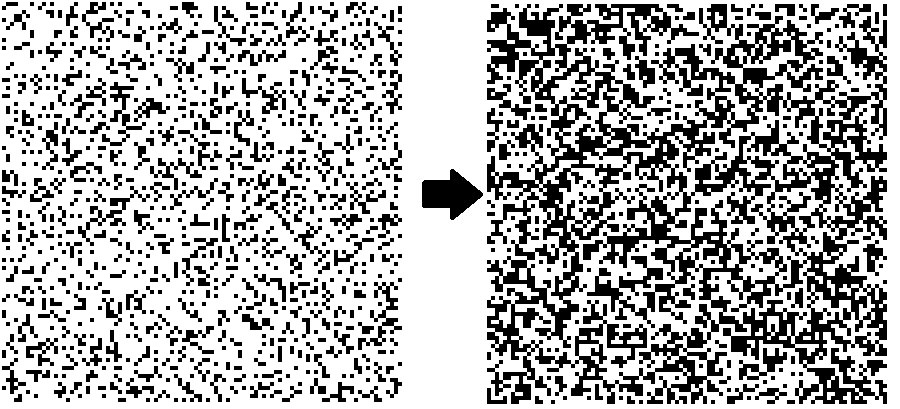
\includegraphics[scale=0.5]{images/imgMargolus/TronAvantApres.png}
        \caption{Algorithme Tron : début aléatoire $\rightarrow$ 1000 générations plus tard}
\end{figure}

\begin{figure}[H]
        \center
        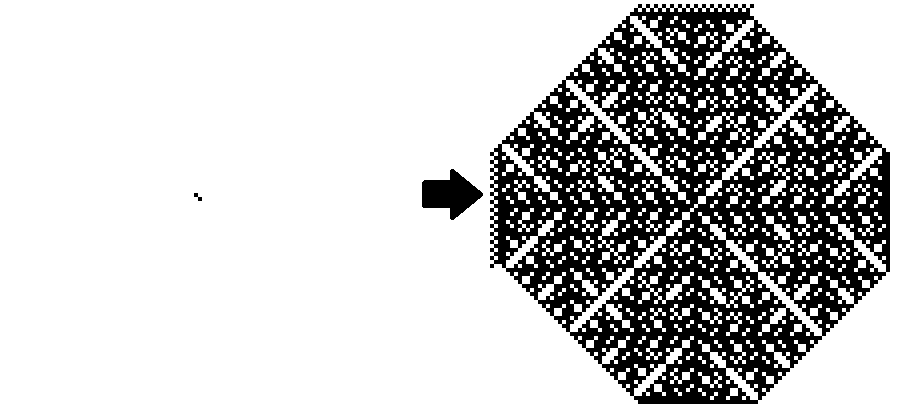
\includegraphics[scale=0.5]{images/imgMargolus/ToothpickAvantApres.png}
        \caption{Algorithme Toothpick : début prédéfini $\rightarrow$ quelques dizaines de générations plus tard}
\end{figure}